% LaTeX Template f�r Datenstrukturen und Algorithmen Abgaben
% Autor: Sandro Speth
% Bei Fragen: Sandro.Speth@studi.informatik.uni-stuttgart.de
\documentclass[12pt]{article}
\usepackage[latin1]{inputenc}
\usepackage[T1]{fontenc}
\usepackage[ngerman]{babel}
\usepackage{graphicx}
\usepackage{color}
\usepackage{listings}
\usepackage[a4paper,lmargin={2cm},rmargin={2cm},tmargin={3.5cm},bmargin = {2.5cm},headheight = {4cm}]{geometry}
\usepackage{amsmath,amssymb,amstext}
\usepackage{amsthm}
\usepackage[lined,algonl,boxed]{algorithm2e}
\usepackage{tikz}
\usepackage[inline]{enumitem}
\usepackage{fancyhdr}
%\usepackage{adjustbox}
\pagestyle{fancy} 
\fancyhf{}

\renewcommand{\theenumi}{(\alph{enumi})}
\renewcommand{\labelenumi}{\text{\theenumi}}

\newcounter{sheetnr}
\setcounter{sheetnr}{8} % Nummer des �bungsblattes

\newcounter{exnum}
\setcounter{exnum}{1} % Nummer der Aufgabe

\newcommand{\aufgabe}[1]{\section*{Aufgabe \theexnum\stepcounter{exnum}: #1}} % Befehl f�r Aufgabentitel

% Rechter Teil der Kopfzeile:
% Namen und Matrikelnummern aller Bearbeiter
\rhead{Wilhelm Buchm�ller(3133783)\\
Daniel Wanner(3149308)\\
Artur Frenzen(2736424)}

% Linker Teil der Kopfzeile
\lhead{Datenstrukturen \& Algorithmen\\
Sommersemester 2016\\
�bungsblatt \thesheetnr}

% Beginn des eigentlichen Dokuments
\begin{document}
% Aufgabe 2
\aufgabe{Dijkstra-Algorithmus}
\begin{enumerate}
\item  \text{}\\
	
\begin{tabular}{l*{6}{c}r}
   Schritt    &         Kosten \\
-         				& A & B & C & D & E  & F \\
\hline
Initialisierung   & 0 & $\infty$ & $\infty$ & $\infty$ & $\infty$ & $\infty$ \\
1          & 0 & 3 & 8 & $\infty$ &  13 & $\infty$     \\
2          & 0 & 3 & 8 & $\infty$ &  13 & 18  \\
3			     & 0 & 3 & 8 & 10 &  13 & 18  \\
4			     & 0 & 3 & 8 & 10 &  13 & 16  \\
5			     & 0 & 3 & 8 & 10 &  12 & 16  \\
\end{tabular}


\item \text{}\\
%TODO:DONE !
		\begin{tikzpicture}
		\begin{scope}[every node/.style={circle,thick,draw}]
			\node (1) at (0,0) {A};
			\node (2) at (-2,1) {B};
			\node (3) at (0,3) {C};
			\node (4) at (6,3) {D};
			\node (5) at (6,0) {E};
			\node (6) at (8,1) {F};
		\end{scope}

	\begin{scope}[>={stealth[black]},
              every node/.style={fill=white,circle},
              every edge/.style={draw=black,very thick}]
              
  \path (2) edge  node {$3$} (1);
	\path (2) edge node {$5$} (3);    
	\path (4) edge  node {$2$}(5);
	\path (4) edge  node {$6$}(6);
	\path (3) edge  node {$2$}(4);
		
    
\end{scope}
\end{tikzpicture}
\end{enumerate}


% Aufgabe 2
\aufgabe{Delaunay-Triangulierung}
% Teilaufgaben
\begin{enumerate}
	\item \text{}\\
	
	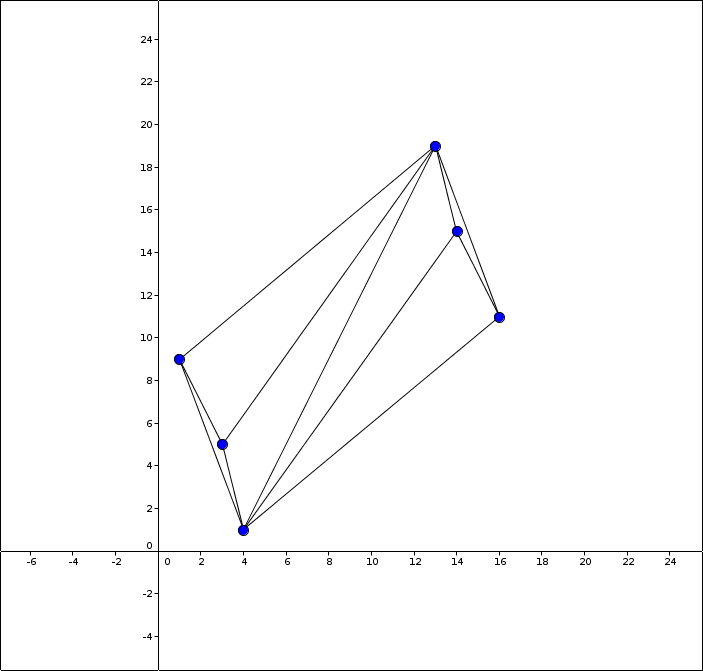
\includegraphics[scale=0.35]{ex08.03/2.png}%
	
	Dies ist eine initiale Triangulierung die mit dem "`Plane-Sweep"'-Verfahren erstellt wurde.
	
	\item
	Aus der Triangulation aus Teilaufgabe a) soll jetzt eine Delaunay-Triangulation erstellt werden.
	Zu Begin werden alle Kanten, welche die Delaunay Eigenschaft verletzen auf auf einen Stack geschoben, in diesem Fall rot markiert.
	%\newpage	%TODO:rauskommentieren falls nicht mehr ben�tigt
	\begin{itemize}
		\item \text{}\\
		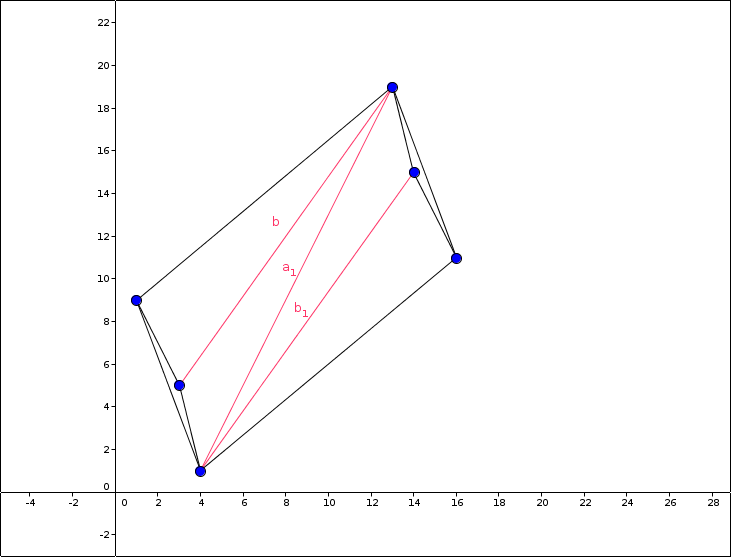
\includegraphics[scale=0.45]{ex08.03/4.png}\newline
		Hier sind die Kanten die die Delaunay-Eigenschaft verletzen rot markiert und bereit zur Abarbeitung.
		
		\item  \text{}\\
		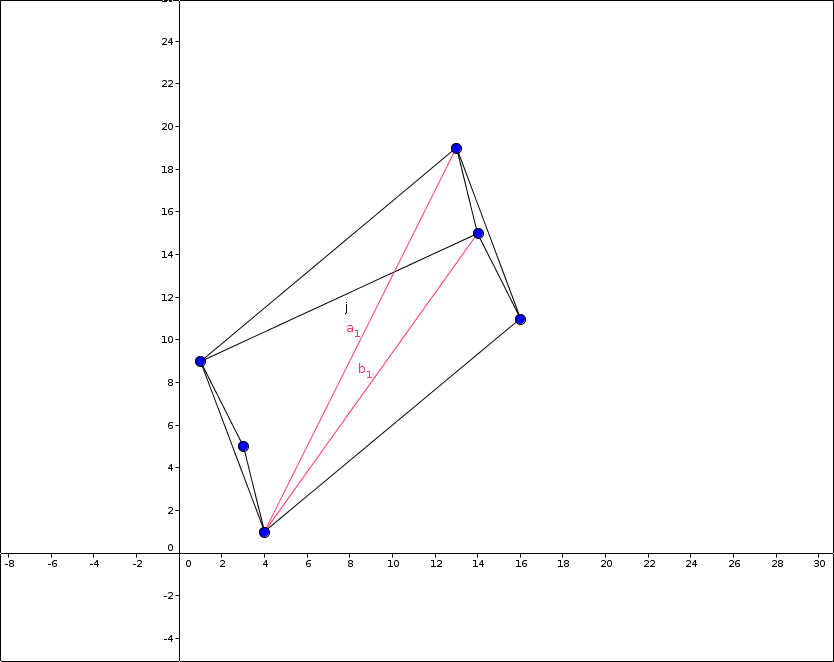
\includegraphics[scale=0.4]{ex08.03/5.png}\newline
		In diesem Schritt wurde die Kante b entfernt und ein "`Edge-Flip"'-Schritt durchgef�hrt, und dadurch die Kante \textit{j} hinzugef�gt.
		Als n�chstes m�ssen wir die Kante \(a_1\) abarbeiten, weil sie zum einen die Delaunay-Eigenschaft verletzt und zum anderen weil \textit{j} , \textit{\(a_1\)} schneidet und somit eine (gedachte) h�here Priorit�t im Stack erh�lt.
		\item  \text{}\\
		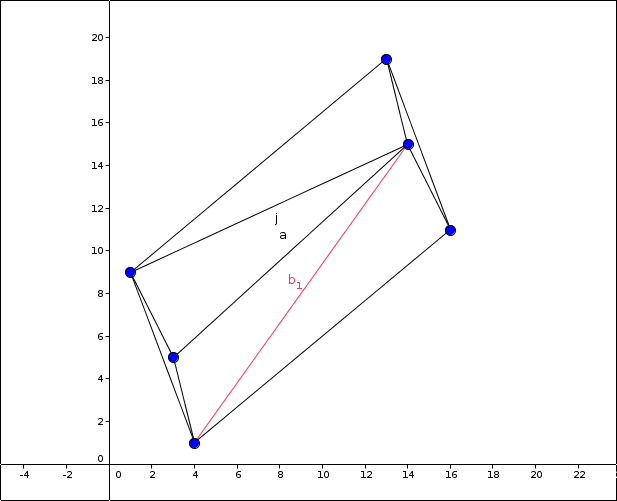
\includegraphics[scale=0.4]{ex08.03/6.png}\newline
		Hier wurde die Kante \(a_1\) entfernt und die Kante a hinzugef�gt. Die Kante \(b_1\) ist die bis jetzt noch die letzte Kante im Stack, wenn durch den "`Edge-Flip"' von \(b_1\) aber weitere Delaunay-Eigenschaften verletzt werden w�chst dieser Stack wieder an.
		\item  \text{}\\
		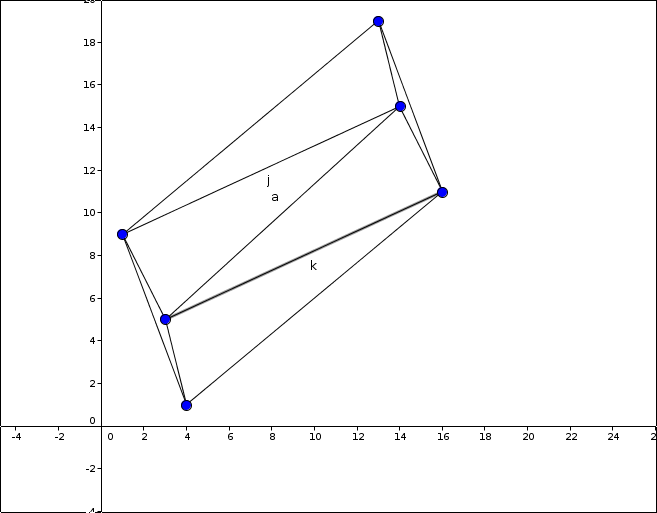
\includegraphics[scale=0.4]{ex08.03/7.png}\newline
		Da keine weiteren Verletzungen geschehen sind, ist unser Graph \textit{G} nun eine Delaunay-Triangulation
	\end{itemize}
\end{enumerate}


% Aufgabe 3
\aufgabe{\framebox[1.1\width]{Impl} in Java}

\paragraph{}\noindent\rule{8cm}{0.4pt}

\aufgabe{Algorithmus von Kruskal}
\aufgabe{Literaturrecherche}
\begin{enumerate}
	\item
	\begin{itemize}
		\item E.W. Dijkstra gibt bei dem erstem Problem zwei Schritte die wiederholt werden bis das Problem gel�st ist
		\item E.W. Dijkstra gibt bei dem zweiten Problem zwei Anmerkungen an
	\end{itemize}
	\item 
	\begin{verbatim}
@article{
    dijkstra1959note,
    title={A note on two problems in connexion with graphs},
    author={Dijkstra, Edsger W},
    journal={Numerische mathematik},
    volume={1},
    number={1},
    pages={269--271},
    year={1959},
    publisher={Springer}
}

    \end{verbatim}
	\item
	\begin{verbatim}
@Article{Dijkstra1959,
    author="Dijkstra, E. W.",
    title="A note on two problems in connexion with graphs",
    journal="Numerische Mathematik",
    year="1959",
    volume="1",
    number="1",
    pages="269--271",
    issn="0945-3245",
    doi="10.1007/BF01386390",
    url="http://dx.doi.org/10.1007/BF01386390"
}

	\end{verbatim}
	\item Da es verschiedene BibTEX-"'Repositories"' gibt, unter anderem auch eine von Google-Scholar und vom Springer-Verlag hat jede Platform eine eigene Style-Convention 
\end{enumerate}
% Ende des Dokuments
\end{document}
